\section{Near Detector and Uncertainties}\label{sec:nu-osc-06}\label{sec:physics-lbnosc-ND}
%{\it Assigned to:} {\bf Chris Marshall} with contributions from Mike Kordosky and Steven Manly and also from Kendall Mahn and Mike Wilking and Justo Martin-Albo.

%This section describes assumptions in the Near Detector simulation and ``reconstruction". Some thought has to go into the connection with the ND CDR and any other ND description in the TDR.



%\begin{itemize}
%    \item The ND concept
%    \item Simulations and ``Reconstruction"
%    \item Event Selections
%    \item Samples
%    \item  Detector Response Systematic Uncertainties
%    \item Connection to Flux and Cross Section Systematic Uncertainty
%    \item DUNE PRISM
%\end{itemize}

\subsection{The Near Detector concept}
\label{sec:ndconcept}

The DUNE near detector (ND) will be located 574 m from the neutrino target at Fermilab and approximately 60 m underground. The hall is oriented at 90 degrees with respect to the beam axis to facilitate measurements at both on-axis and off-axis locations. The detector concept consists of a liquid argon time-projection chamber (LAr TPC) functionally coupled to a magnetized multi-purpose tracker (MPT). The MPT includes a high-pressure gaseous argon (HPG) TPC, surrounded by an electromangetic calorimeter (ECal), and a magnet. What follows is a description of the near detector as implemented in the long baseline oscillation sensitivity analysis described in this chapter. Details of the design are being optimized, and the actual detector may be somewhat different than what is described here. More details on the design can be found in Chapter~\ref{ch:ndexecutivesummary}.

The LAr TPC is a modular, segmented detector based on the concept being studied by the Argon Cube collaboration~\cite{ArgonCube} \fixme{find citation}, and is the most upstream component of the ND. Each module is itself a LAr TPC with two anode planes and a central cathode. The active dimensions are $1 \times 3 \times 1$~m ($x \times y \times z$), where the $z$ direction is $6^{\circ}$ upward from the neutrino beam, and the $y$ direction points upward. Charge drifts in the $\pm x$ direction, with a maximum drift distance of 50 cm for electrons created in the center of a module. The module design is described in detail in Ref.~\cite{ArgonCube?}\fixme{ArCube citation}. The full LAr detector consists of 35 modules in a single cryostat, arranged in an array 5 modules deep in the $z$ direction and 7 modules across in $x$ so that the total active dimensions are $7 \times 3 \times 5$~m. The total active LAr volume is $105 m^{3}$, corresponding to a mass of 147 tons.

The anode planes are tiled with readout pads, such that the $yz$ coordinate is given by the pad location and the $x$ coordinate is given by the drift time, and the three-dimensional position of an energy deposit is uniquely determined~\fixme{ cite larpix jinst}. The module walls orthogonal to the anode and cathode are lined with a photon detector that is sensitive to scintillation light produced inside the module. \fixme{describe arclight better}. The detector is optically segmented, and the tiled ArCLight design gives $\sim$30 cm position resolution in the vertical coordinate, so that light flashes from individual neutrino interactions can be identified. The neutrino interaction time, $t_{0}$, is determined from the prompt component of the scintillation light. Even absent a scintillation signal, the pulsed beam gives $\sim$1.6 cm position resolution in the drift direction.

The MPT sits immediately downstream of the LAr TPC so that in the on-axis position, the beam center crosses the exact center of both the LAr and HPG active volumes. The magnet is a solenoid with an inner radius of 320 cm and total length along the cylinder axis of 780 cm. The axis is oriented at $90^{\circ}$ with respect to the beam, pointing along $x$. The yoke is cut out in the upstream barrel to minimize the passive material between the two TPC detectors. The central field strength is 0.4 T.

The HPG TPC sits inside the magnet in a 3 cm thick cylindrical titanium pressure vessel. The cylindrical TPC radius is 273 cm, and its length along the $x$ axis is 518 cm. It is divided into two drift regions by a central cathode, and filled with a 90/10 Ar/CO$_{2}$ gas mixture. A tiled, fine-grained ECal surrounds the HPG TPC. Each ECal layer consists of a 2 mm copper absorber and an array of $10 \times 10 \times 5$~mm scintillator tiles. Each tile is read out by a SiPM mounted on to a 1 mm thick printed circuit board. The inner-most 10 ECal layers are inside the pressure vessel, with 20 additional layers outside. The tiled design of the inner ECal gives excellent angular resolution to photon-induced showers, enabling vertex reconstruction of $\pi^{0}$s produced inside the gas volume, which typically do not convert in the TPC. The outer ECal primarily serves to contain energy of electromagnetic showers. The ECal design is described in Ref.~\fixme{cite Simon et al. CALICE paper}. \fixme{a bit more detail on the ECal?}

\fixme{Add a visualization of geometry as figure}

\subsection{Simulations and parameterized reconstruction}
% There's a separate tools section, and this is one place which may be factorizable; this can be done by overal TDR editors - KM

\label{sec:ndsimreco}

Neutrino interactions are simulated in the active volumes of the LAr and HPG TPCs described in Section~\ref{sec:ndconcept}. The neutrino flux prediction is described in Section~\ref{ch:osc-bm-nus}.%\label{sec:nu-osc-05}
Interactions are simulated with the GENIE event generator using the model configuration described in Section~\ref{sec:nu-osc-05}. The propagation of neutrino interaction products through the detector volumes is simulated using a Geant4-based model. Pattern recognition and reconstruction software has not yet been developed for the near detector. Instead, we perform a parameterized reconstruction based on true energy deposits in active detector volumes as simulated by Geant4.

The LAr fiducial region is a central $6 \times 2 \times 3$~m$^{3}$~volume with a 50 cm active buffer on the sides and upstream end, and a 150 cm active buffer on the downstream end. Hadronic energy is estimated from energy deposits in the active LAr volume only. \fixme{probably times some multiplier in the future} A veto region is defined as the outer 30 cm of the active volume on all sides. Events with more than 30 MeV total energy deposit in the veto region are excluded from analysis, as this energy near the detector edge suggests leakage, resulting in poor energy reconstruction. Even with the containment requirement, events with large shower fluctuations to neutral particles can still be very poorly reconstructed. Neutrons, in particular, are largely unreconstructed energy.

Electrons are reconstructed calorimetrically in the liquid argon. The radiation length is 14 cm in LAr, so for fiducial interactions there are between 10 and 30 radiation lengths between the vertex and the edge of the TPC. As there is no magnetic field in the LAr TPC region, electrons and positrons cannot be distinguished.

Muons with kinetic energy greater than $\sim$1 GeV typically exit the LAr. An energetic forward-going muon will pass through the ECal and into the gaseous TPC, where its momentum and charge are reconstructed by curvature. For these events, it is possible to differentiate between $\mu^{+}$ and $\mu^{-}$ event by event. Muons that stop in the LAr or ECal are reconstructed by range. Exiting muons that do not match to the HPG TPC are not reconstructed, and events with these tracks are rejected from analysis. The asymmetric transverse dimensions of the LAr volume make it possible to reconstruct wide-angle muons with some efficiency. High-angle tracks are typically lost when the $\nu-\mu$ plane is nearly parallel to the $y$ axis, but are often contained when it is nearly parallel to the $x$ axis. 

The charge of stopping muons in the LAr volume cannot be determined. However, the wrong-sign flux is predominantly concentrated in the high-energy tail, where leptons are likelier to be forward and energetic. In FHC mode, the wrong-sign background in the focusing peak is negligibly small, and $\mu^{-}$ is assumed for all stopping muon tracks. In RHC mode, the wrong-sign background is larger in the peak region. Furthermore, high-angle leptons are generally at higher inelasticity, which enhances the wrong-sign contamination in the contained muon sample. To mitigate this, a Michel electron is required. The wrong-sign $\mu^{-}$ captures on Ar with 75\% probability, effectively suppressing the relative $\mu^{-}$ component by a factor of four.

\fixme{all of this may change as we update the cheated reco}
Events are classified as either $\nu_{\mu}$ CC, $\bar{\nu}_{\mu}$ CC, $\nu_{e}$+$\bar{\nu}_{e}$ CC, or NC. True muons and charged pions are evaluated as potential muon candidates. The track length is determined by following the true particle trajectory until it hard scatters or ranges out. The particle is classified as a muon if its track length is at least 1 m, and the mean energy deposit per centimeter of track length is less than 3 MeV. The mean energy cut rejects tracks with detectable hadronic interactions. The minimum length requirement imposes an effective threshold on true muons of about 200 MeV kinetic energy, but greatly suppresses potential NC backgrounds with short, non-interacting charged pions.

True electrons are reconstructed with an ad-hoc efficiency that is zero below 300 MeV, and rises linearly to unity between 300 and 700 MeV. Neutral-current backgrounds arise from photon and $\pi^{0}$ production. Photons are misreconstructed as electrons when the energy deposit per centimeter in the first few cm after conversion is less than 4 MeV. This is typically for Compton scatters, and can also occur due to a random downward fluctuation in the $e^{+}e^{-}$ dE/dx. The conversion distance must also be small so that no visible gap can be identified. We consider a photon gap to be clear when the conversion distance is greater than 2cm, which corresponds to at least three pad widths. For $\pi^{0}$ events, the second photon must also be either less than 50 MeV, or have an opening angle to the first photon less than 10 mrad. It is possible for CC $\nu_{\mu}$ events to be reconstructed as CC $\nu_{e}$ when the muon is too soft and a $\pi^{0}$ fakes the electron.

\fixme{Gas TPC sample description will go here.}

\subsection{Event Selections, Samples}

Events are classified as $\nu_{\mu}$ CC, $\bar{\nu}_{\mu}$ CC, $\nu_{e}$ + $\bar{\nu}_{e}$ CC, or NC. Charged-current events are required to have exactly one reconstructed lepton of the apropriate flavor. The muon-flavor samples are separated by reconstructed charge, but the electron sample is combined because the charge cannot be determined. The neutral-current sample includes all events with zero reconstructed leptons.

Events with exiting tracks that do not enter the HPG TPC are rejected. These are predominantly muon CC, where the muon momentum cannot be determined. Events with more than 30 MeV of visible hadronic energy in the veto region are also excluded.

\begin{figure}
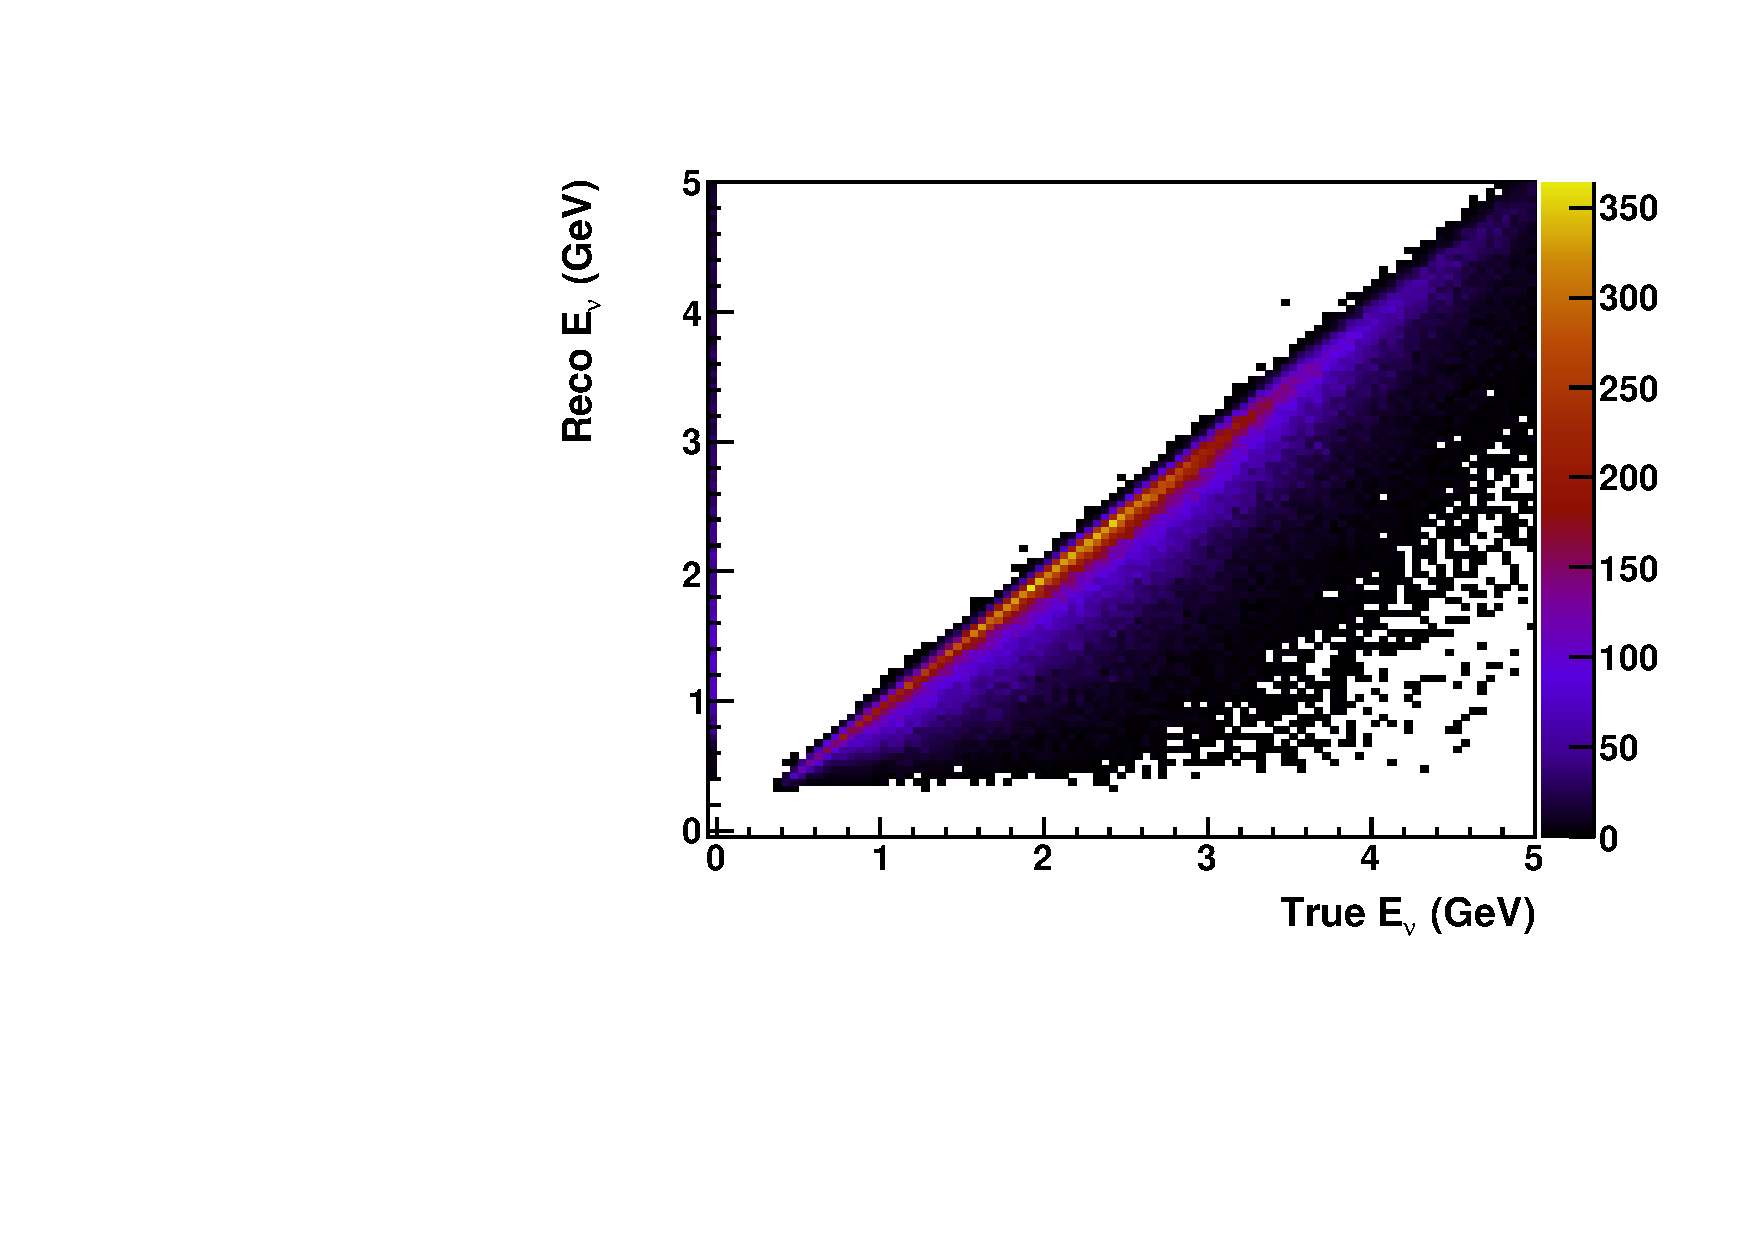
\includegraphics[width=\textwidth]{graphics/true_reco_Ev.pdf}
\caption{Placeholder: reconstructed vs. true neutrino energy for $\nu_{\mu}$ CC events with either contained or MPT-matched muon and ell-contained hadronic shower. The bin at zero true energy corresponds to events that are not true $\nu_{\mu}$ CC, which are mostly neutral current with a charged pion faking the muon track, hence the lower energy spectrum.}
\label{fig:truerecoEv}
\end{figure}

\begin{figure}
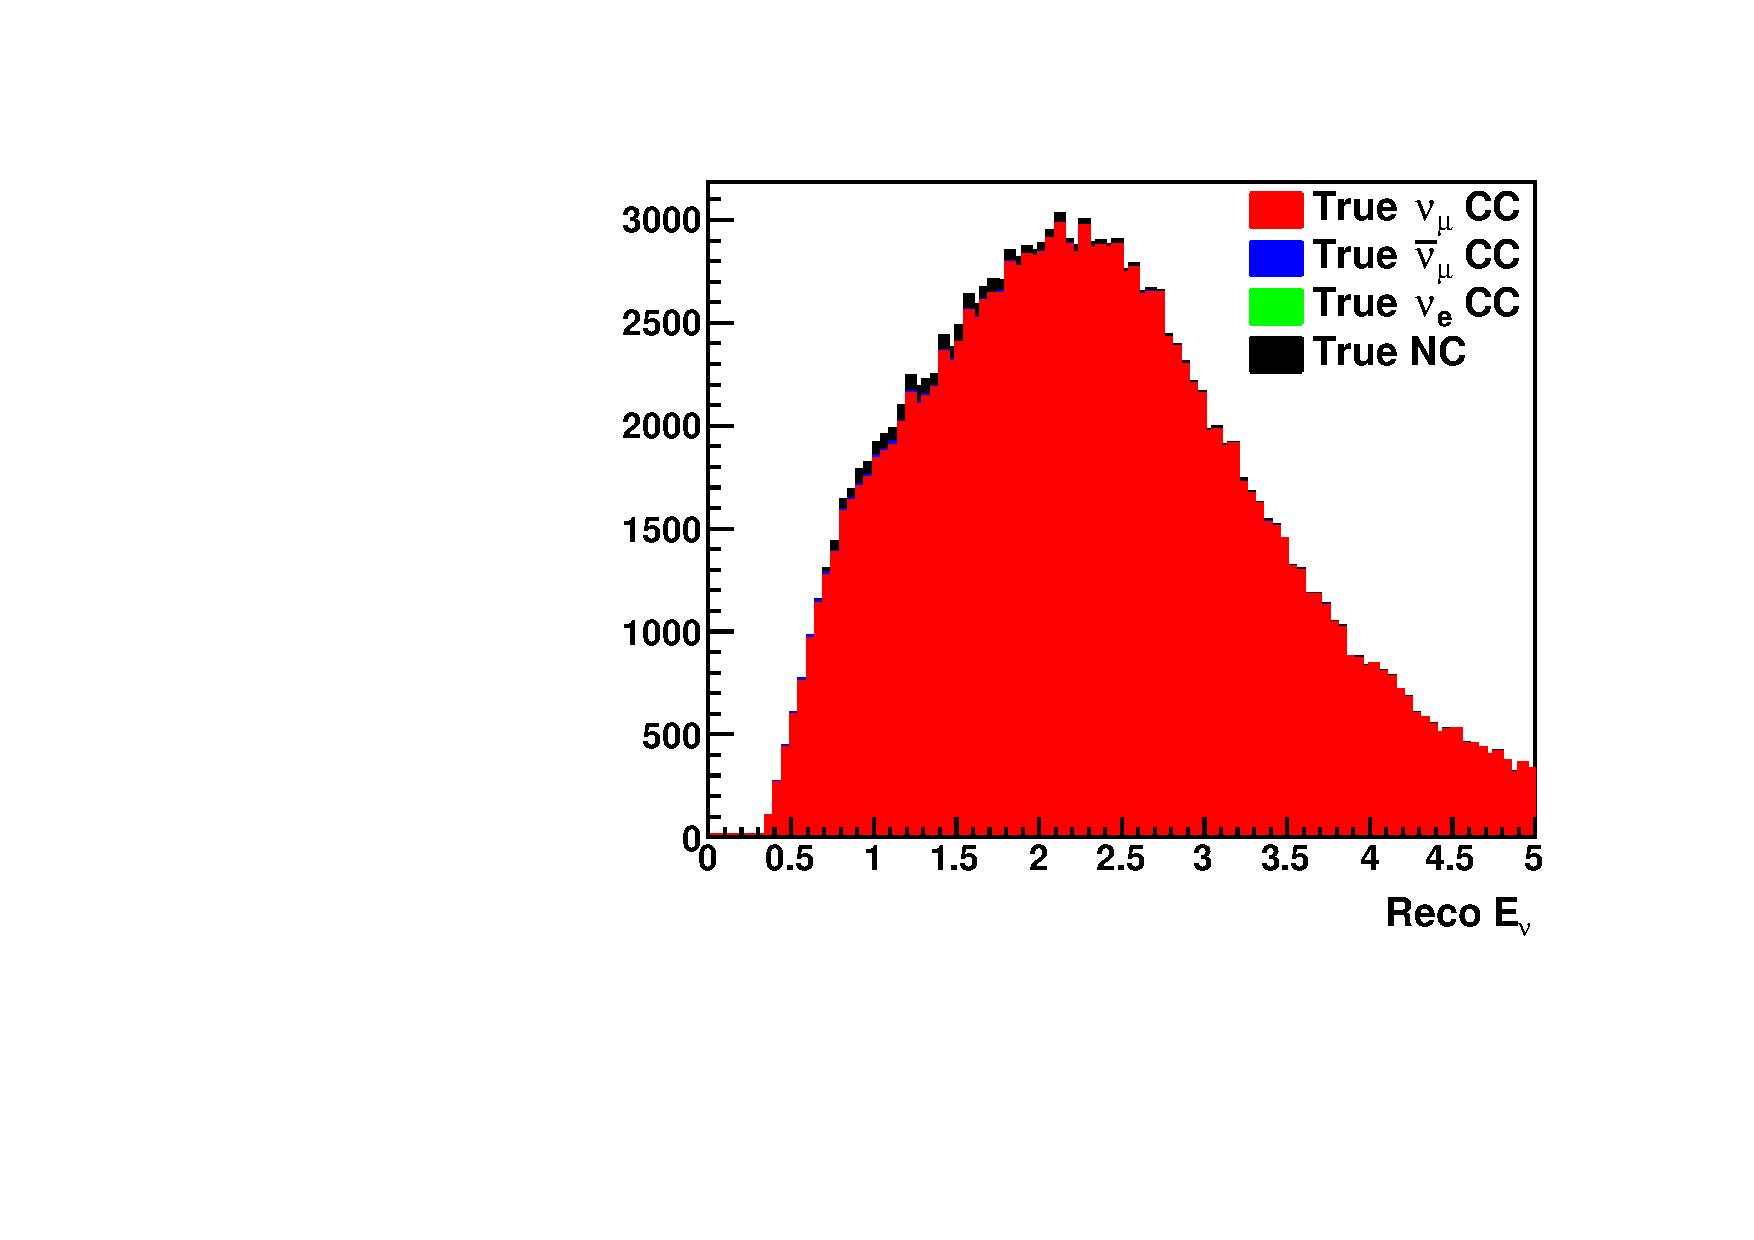
\includegraphics[width=0.3\textwidth]{graphics/recoE_muCC.pdf}
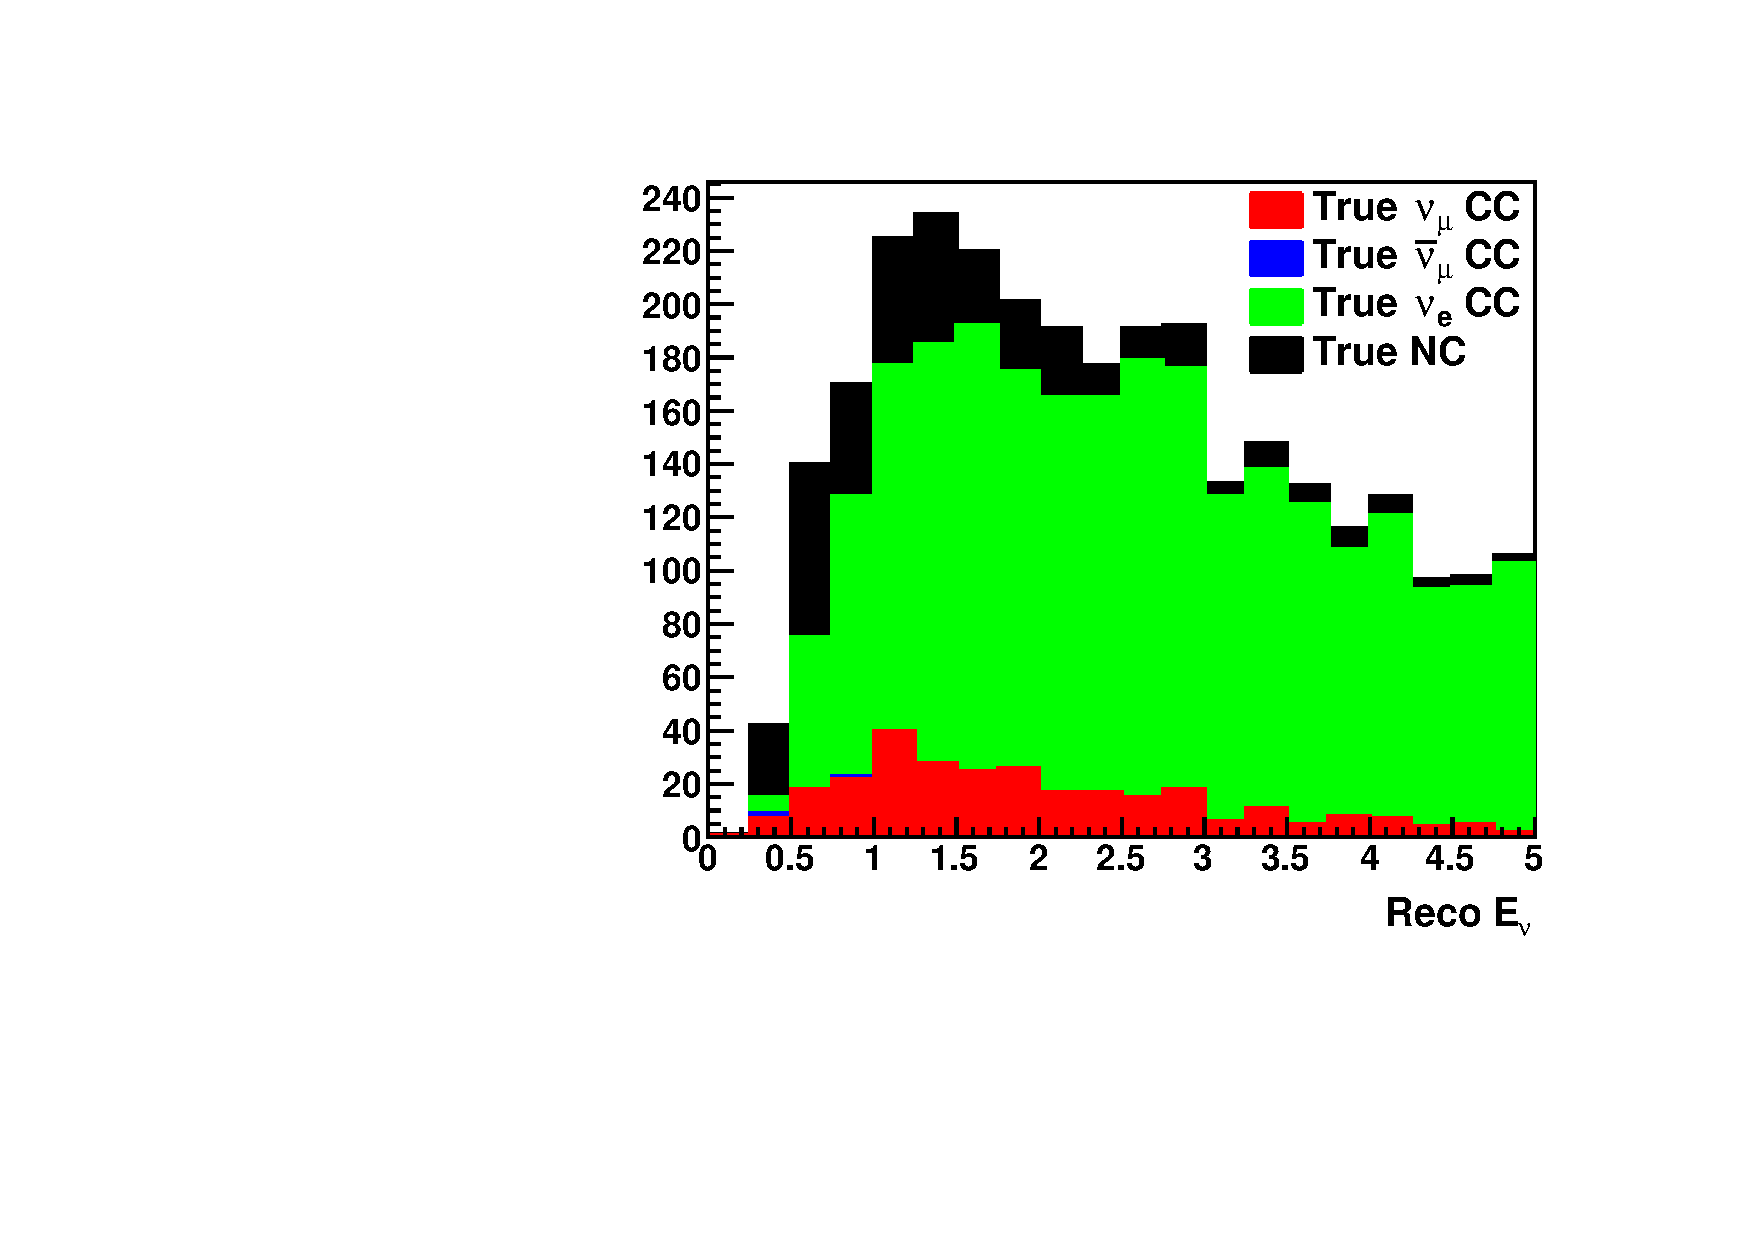
\includegraphics[width=0.3\textwidth]{graphics/recoE_eCC.pdf}
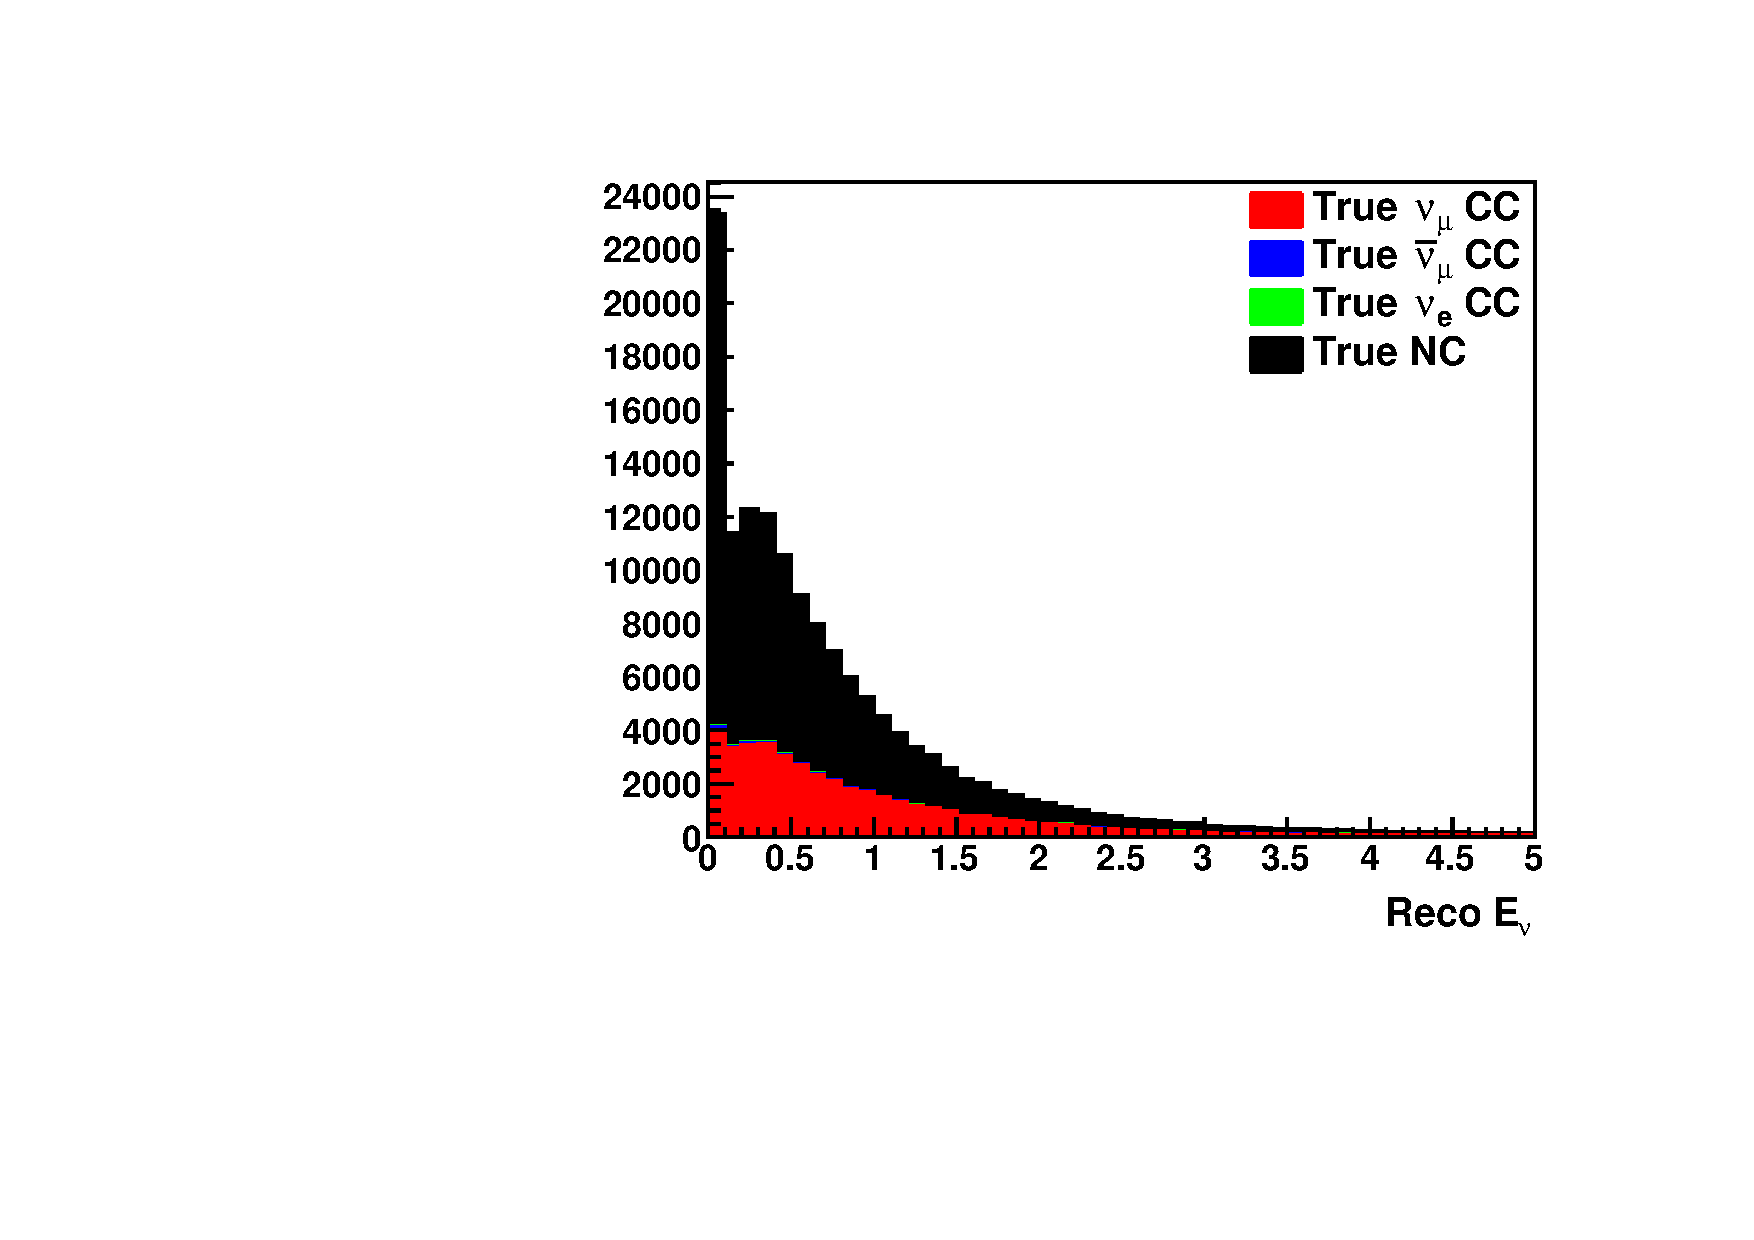
\includegraphics[width=0.3\textwidth]{graphics/recoE_NC.pdf}
\caption{Reconstructed neutrino energy for events classified as $\nu_{\mu}$ CC, $\nu_{e}$ CC, and NC in FHC mode. The colors correspond to true neutrino flavor.}
\label{fig:recoEvcats}
\end{figure}

\fixme{plots of acceptance vs. kinematics}

Selection in an off-axis location of the LAr detector is similar to the on-axis case. The event rate, after selection, is shown as a function of off-axis position in Table~\ref{table:evrates_LAR}.  The predictions are POT-scaled to an illustrative year-long run plan that takes 50\% of the available POT on-axis spreads the remaining beam time equally among  twelve off-axis positions. \fixme{Update text to run plan you want to see current approximate number  of positions?} 


\todo{Update numbers for table: LAr  event rates in slices of off-axis position.}

\begin{table}
\begin{tabular}{ l l || c c | c || c c | c | c || c }
\multirow{3}{*}{Offset} & \multirow{3}{*}{$10^{19}$POT} & \multicolumn{7}{c||}{CCInc} & NCInc \\
\cline{3-10}
& & \multicolumn{3}{c||}{$\mu$ contained} & \multicolumn{3}{c|}{$\mu$ exit, $\textrm{T}_{\mu}^\textrm{\tiny exit} > 50 \textrm{MeV}$} & \multirow{2}{*}{$\nu_\textrm{e}$} & \multirow{2}{*}{$\nu_{\mu}$} \\
& & $\nu_{\mu}$ & $\epsilon_{\nu_{\mu},\textsc{cc}}$ & $\bar{\nu}_{\mu}$/$\nu_{\mu}$ & $\nu_{\mu}$ & $\epsilon_{\nu_{\mu},\textsc{cc}}$ & $\bar{\nu}_{\mu}$/$\nu_{\mu}$ & & \\ \hline
 0~m  &  55  & 6.6E5 & 3\% & 1\% & 5.3E6 & 22\% & 3\% & 6.2E4 & 1.8E6 \\
 3~m  &  4.58  & 5.5E4 & 3\% & 1\% & 4.1E5 & 22\% & 3\% & 5.0E3 & 1.4E5  \\
 6~m  &  4.58  & 5.8E4 & 4\% & 1\% & 3.0E5 & 22\% & 4\% & 4.3E3 & 1.1E5 \\
 9~m  &  4.58  & 6.0E4 & 7\% & 2\% & 1.9E5 & 22\% & 4\% & 3.4E3 & 7.5E4 \\
 12~m  &  4.58  & 5.9E4 & 12\% & 3\% & 1.1E5 & 22\% & 5\% & 2.5E3 & 5.2E4 \\
 15~m  &  4.58  & 5.4E4 & 18\% & 3\% & 6.2E4 & 20\% & 6\% & 2.2E3 & 3.7E4 \\
 18~m  &  4.58  & 4.6E4 & 22\% & 4\% & 3.8E4 & 18\% & 8\% & 1.7E3 & 2.7E4 \\
 21~m  &  4.58  & 3.9E4 & 27\% & 5\% & 2.5E4 & 17\% & 9\% & 1.4E3 & 2.1E4 \\
 24~m  &  4.58  & 3.1E4 & 30\% & 6\% & 1.7E4 & 16\% & 9\% & 1.2E3 & 1.6E4 \\
 27~m  &  4.58  & 2.6E4 & 32\% & 7\% & 1.2E4 & 15\% & 10\% & 9.8E2 & 1.3E4 \\
 30~m  &  4.58  & 2.1E4 & 33\% & 7\% & 9.6E3 & 16\% & 12\% & 8.3E2 & 1.0E4 \\
 33~m  &  4.58  & 1.7E4 & 35\% & 8\% & 7.5E3 & 15\% & 13\% & 7.6E2 & 8.3E3 \\
 36~m  &  4.58  & 1.2E4 & 35\% & 8\% & 6.1E3 & 16\% & 15\% & 6.7E2 & 6.6E3 \\
\hline
\hline
\multicolumn{2}{c||}{Totals} & $\nu_{\mu}$ & --- & $\bar{\nu}_{\mu}$ & $\nu_{\mu}$ & --- & $\bar{\nu}_{\mu}$ & $\nu_\textrm{e}$ & $\nu_{\mu}$ \\ \hline
 All  &  110  & 1.1E6 & --- & 1.6E4 & 6.5E6 & --- & 2.2E5 & 8.7E4 & 2.3E6 \\
\end{tabular}

\caption{The selected event rates for a year-long, neutrino-mode run plan. The wrong sign fraction, intrinsic electron neutrino and neutral current event rates are also shown. In all cases, the hadronic containment cut is applied, and the (anti-)muon neutrino events are separated into two samples depending on the containment topology of the final state muon.}
\label{table:evrates_LAR}
\end{table}

The efficiency to select events in an off-axis position varies in a well-defined way based on muon range, angle and hadronic system. Interactions that occur near the edge of the LAr fiducial region produce muons that are more likely to exit the detector volume with sufficient kinetic energy than those occurring in the center of a detector; at increasingly larger off-axis positions, the lower average energy of the neutrino beam produces more contained muons. Even though the neutrino energy spectra varies significantly as a function of off-axis angle, the efficiency for containing the hadronic system only depends on the fractional energy transferred to the hadronic system, as expected. \fixme{Mike: Please clean up this text}

\fixme{Add gas TPC selections}

One outcome of the ND process will be to determine if the MPT will move with the LAr detector. For this document, rates of the LAr are presented in Table~\ref{table:evrates_LAR} are separated based on whether or not the muon is contained (and there is an MPT). Regardless, the table shows that it will be possible to collect sufficient statistics in all off-axis positions with a run plan in which 50\% of the data is collected with the detector in the on-axis position. 

\subsection{Detector Response Systematic Uncertainties}

\todo{Write ND detector response systematic uncertainties}

\subsection{Role of Near detector in flux and cross section systematic uncertainty assessment}
% Connection to Flux and Cross Section Systematic Uncertainty

 The selected charged-current on- and off-axis samples are fit in two-dimensional bins of neutrino energy, $E_{\nu} = E_{lep} + E_{had}$, and inelasticity, $y = E_{had}/E_{\nu}$ to constrain nuisance parameters associated to the flux and interaction model. Due to significant correlations in the flux at the on-axis position and  cross section physics (same target material) the on-axis event samples are expected to reduce the overall flux and cross section uncertainty by approximately a factor of two. The off-axis event samples will have comparable constraint, and so can serve as a test of the interaction model and/or flux model. The off-axis positions are sensitive to changes of the focusing optics (e.g. horn current or position), and studies demonstrate that the off-axis positions event rates are valuable to diagnose incomplete aspects of the cross section model.

In addition to the analysis presented here, DUNE will employ a range of additional techniques and samples to further constrain the flux and cross section uncertainties: \begin{itemize}
\item Neutrino-electron elastic scattering is a rare process with a well know cross section. A dedicated selection, following work with a comparable flux%Citation: https://inspirehep.net/record/1411311
, can be used to reduce the flux uncertainties.
\item Low-nu method?
\item Alternate projections of the data, such as Ref~%http://inspirehep.net/record/1410087
or exclusive selections separated by final state particles, may be
 used to constrain cross section physics.
\end{itemize}

\subsubsection{Neutrino-electron elastic scattering}
\label{sec:nu+e}

Measurements of neutrino-nucleus scattering are sensitive to the product of the flux and cross section, both of which are uncertain. This can lead to a degeneracy between flux and cross section nuisance parameters in the oscillation fit, and result in significant anti-correlations, even when the uncertainty on the diagonal component is small. One way to break this degeneracy is by including a sample for which the a priori cross section uncertainties are very small. 

Neutrino-electron scattering is a pure-electroweak process with calculable cross section at tree level. The final state consists of a single electron, subject to the kinematic limit 

\begin{equation}
1 - \cos \theta = \frac{m_{e}(1-y)}{E_{e}},
\end{equation}

where $\theta$ is the angle between the electron and incoming neutrino, $E_{e}$ and $m_{e}$ are the electron mass and total energy, respectively, and $y = T_{e}/E_{\nu}$ is the fraction of the neutrino energy transferred to the electron. For DUNE energies, $E_{e} \gg m_{e}$, and the angle $\theta$ is very small, such that $E_{e}\theta^{2} < 2m_{e}$.

The overall flux normalization can be determined by counting $\nu e \rightarrow \nu e$ events. Events can be identified by searching for a single electromagnetic shower with no other visible particles. Backgrounds from $\nu_{e}$ charged-current scattering can be rejected by looking for large energy deposits near the interaction vertex, which are evidence of nuclear breakup. Photon-induced showers from neutral-current $\pi^{0}$ events can be distinguished from electrons by the energy profile at the start of the track. The dominant background is expected to be $\nu_{e}$ charged-current scattering at very low $Q^{2}$, where final-state hadrons are below threshold, and $E_{e}\theta^{2}$ happens to be small. The background rate can be constrained with a control sample at higher $E_{e}\theta^{2}$, but the shape extrapolation to $E_{e}\theta^{2} \rightarrow 0$ is uncertain at the 10-20\% level.

For the DUNE flux, approximately 100 events per year per ton of fiducial mass ar expected with electron energy above 0.5 GeV. For a LAr TPC mass of 25 tons, this corresponds to 2500 events per year, or 12500 events in the full 5-year FHC run, assuming the ND stays on axis. Given the very forward signal, it may be possible to expand the fiducial volume to enhance the rate. The statistical uncertainty on the flux normalization from this technique is expected to be $\sim$1\%.



